%
% nurimaze.tex
%
% (c) 2019 Prof Dr Andreas Müller, Hochschule Rapperswil
%
\documentclass[tikz]{standalone}
\usepackage{times}
\usepackage{txfonts}
\usepackage[utf8]{inputenc}
\usepackage{graphics}
\usepackage{ifthen}
\usepackage{color}
\usetikzlibrary{arrows,intersections}
\usetikzlibrary{math}
\begin{document}


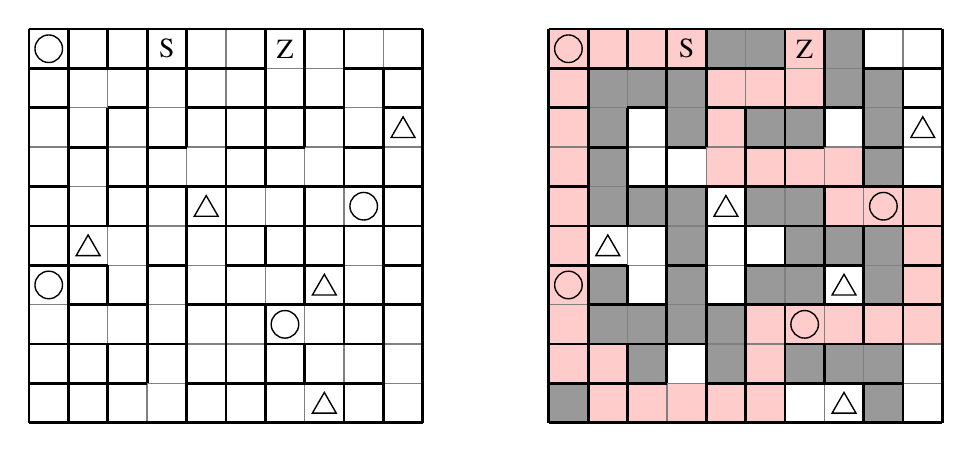
\begin{tikzpicture}[>=latex,thick]

\def\sk{0.5}
\def\cc#1{\draw[line width=0.5pt] #1 circle[radius={0.35*\sk}];}
\def\triangle#1#2{
\begin{scope}[yshift=-0.04cm]
	\draw[line width=0.5pt]
		({#1+0.35*\sk*cos(-30)},{#2+0.35*\sk*sin(-30)})--
		({#1+0.35*\sk*cos(90)},{#2+0.35*\sk*sin(90)})--
		({#1+0.35*\sk*cos(210)},{#2+0.35*\sk*sin(210)})--cycle;
\end{scope}
}
\def\rosa#1#2{
\fill[color=red!20] ({#1*\sk},{#2*\sk})-- ({(#1+1)*\sk},{#2*\sk})--
	({(#1+1)*\sk},{(#2+1)*\sk})-- ({#1*\sk},{(#2+1)*\sk})--cycle;
}
\def\grau#1#2{
\fill[color=black!40] ({#1*\sk},{#2*\sk})-- ({(#1+1)*\sk},{#2*\sk})--
	({(#1+1)*\sk},{(#2+1)*\sk})-- ({#1*\sk},{(#2+1)*\sk})--cycle;
}

\def\hlinie#1#2#3{
\draw[line width=1pt] ({#1*\sk},{#3*\sk})--({#2*\sk},{#3*\sk});
}
\def\vlinie#1#2#3{
\draw[line width=1pt] ({#1*\sk},{#2*\sk})--({#1*\sk},{#3*\sk});
}

\def\allrosa{
\rosa{0}{1}
\rosa{0}{2}
\rosa{0}{3}
\rosa{0}{4}
\rosa{0}{5}
\rosa{0}{6}
\rosa{0}{7}
\rosa{0}{8}
\rosa{0}{9}

\rosa{1}{0}
\rosa{1}{1}
\rosa{1}{9}

\rosa{2}{0}
\rosa{2}{9}

\rosa{3}{0}
\rosa{3}{9}

\rosa{4}{0}
\rosa{4}{6}
\rosa{4}{7}
\rosa{4}{8}

\rosa{5}{0}
\rosa{5}{1}
\rosa{5}{2}
\rosa{5}{6}
\rosa{5}{8}

\rosa{6}{2}
\rosa{6}{6}
\rosa{6}{8}
\rosa{6}{9}

\rosa{7}{2}
\rosa{7}{5}
\rosa{7}{6}

\rosa{8}{2}
\rosa{8}{5}

\rosa{9}{2}
\rosa{9}{3}
\rosa{9}{4}
\rosa{9}{5}
}

\def\allgrau{
\grau{0}{0}

\grau{1}{2}
\grau{1}{3}
\grau{1}{5}
\grau{1}{6}
\grau{1}{7}
\grau{1}{8}

\grau{2}{1}
\grau{2}{2}
\grau{2}{5}
\grau{2}{8}

\grau{3}{2}
\grau{3}{3}
\grau{3}{4}
\grau{3}{5}
\grau{3}{7}
\grau{3}{8}

\grau{4}{1}
\grau{4}{2}
\grau{4}{9}

\grau{5}{3}
\grau{5}{5}
\grau{5}{7}
\grau{5}{9}

\grau{6}{1}
\grau{6}{3}
\grau{6}{4}
\grau{6}{5}
\grau{6}{7}

\grau{7}{1}
\grau{7}{4}
\grau{7}{8}
\grau{7}{9}

\grau{8}{0}
\grau{8}{1}
\grau{8}{3}
\grau{8}{4}
\grau{8}{6}
\grau{8}{7}
\grau{8}{8}
}

\def\feld{
\foreach \x in {0,1,...,10}{
	\draw[color=gray,line width=0.5pt] ({\x*\sk},0)--({\x*\sk},{10*\sk});
	\draw[color=gray,line width=0.5pt] (0,{\x*\sk})--({10*\sk},{\x*\sk});
}
\draw[line width=1pt] (0,0)--({10*\sk},0);
\draw[line width=1pt] (0,{10*\sk})--({10*\sk},{10*\sk});
\draw[line width=1pt] (0,0)--(0,{10*\sk});
\draw[line width=1pt] ({10*\sk},0)--({10*\sk},{10*\sk});

\cc{({0.5*\sk},{3.5*\sk})}
\cc{({0.5*\sk},{9.5*\sk})}
\cc{({6.5*\sk},{2.5*\sk})}
\cc{({8.5*\sk},{5.5*\sk})}

\triangle{1.5*\sk}{4.5*\sk}
\triangle{4.5*\sk}{5.5*\sk}
\triangle{7.5*\sk}{0.5*\sk}
\triangle{7.5*\sk}{3.5*\sk}
\triangle{9.5*\sk}{7.5*\sk}

\node at ({3.5*\sk},{9.5*\sk}) {S};
\node at ({6.5*\sk},{9.5*\sk}) {Z};

\hlinie{0}{3}{1}
\hlinie{4}{9}{1}
\hlinie{0}{4}{2}
\hlinie{6}{9}{2}
\hlinie{1}{3}{3}
\hlinie{4}{10}{3}
\hlinie{0}{2}{4}
\hlinie{3}{4}{4}
\hlinie{5}{8}{4}
\hlinie{9}{10}{4}
\hlinie{0}{3}{5}
\hlinie{4}{10}{5}
\hlinie{0}{1}{6}
\hlinie{2}{10}{6}
\hlinie{1}{2}{7}
\hlinie{3}{4}{7}
\hlinie{5}{7}{7}
\hlinie{8}{9}{7}
\hlinie{0}{1}{8}
\hlinie{2}{3}{8}
\hlinie{4}{8}{8}
\hlinie{9}{10}{8}
\hlinie{0}{6}{9}
\hlinie{8}{10}{9}

\vlinie{1}{0}{10}
\vlinie{2}{0}{2}
\vlinie{2}{3}{4}
\vlinie{2}{5}{8}
\vlinie{2}{9}{10}
\vlinie{3}{1}{10}
\vlinie{4}{0}{6}
\vlinie{4}{7}{10}
\vlinie{5}{0}{8}
\vlinie{6}{0}{3}
\vlinie{6}{4}{5}
\vlinie{6}{6}{10}
\vlinie{7}{1}{2}
\vlinie{7}{3}{6}
\vlinie{7}{7}{10}
\vlinie{8}{0}{1}
\vlinie{8}{2}{5}
\vlinie{8}{6}{10}
\vlinie{9}{0}{9}
}

\begin{scope}[xshift=-3.3cm]
\feld
\end{scope}

\begin{scope}[xshift=3.3cm]
\allgrau
\allrosa
\feld
\end{scope}

\end{tikzpicture}

\end{document}
